\documentclass[9pt,aspectratio=169]{beamer}

% ============ FONTS ============
\usepackage{fontspec}
\setmainfont{Latin Modern Sans}
\newfontfamily\headingfont{Poppins}
\newfontfamily\poppinslight{Poppins Light}
\setmonofont{DejaVu Sans Mono}[Scale=0.82]

\usepackage{amsmath,amssymb,amsthm}
\usepackage{tikz}
\usetikzlibrary{positioning,shapes.geometric,arrows.meta,decorations.pathmorphing,calc,fit,backgrounds}
\usepackage{booktabs}
\usepackage{array}
\usepackage{listings}
\usepackage{xcolor}

% ============ COLOR PALETTE : "Deep Reef" ============
\definecolor{reefInk}{HTML}{0A2E36}      % near-black teal, backgrounds
\definecolor{reefDeep}{HTML}{0E3B45}     % deep teal
\definecolor{reefMid}{HTML}{146671}      % mid teal
\definecolor{reefBright}{HTML}{1FA6A6}   % bright teal accent
\definecolor{reefGold}{HTML}{E3A857}     % warm gold accent
\definecolor{reefCoral}{HTML}{E4694A}    % coral, sparing use
\definecolor{reefSand}{HTML}{F4EFE6}     % warm off-white
\definecolor{reefGrey}{HTML}{5B6B6E}     % muted body grey

\setbeamercolor{normal text}{fg=reefInk,bg=reefSand}
\setbeamercolor{structure}{fg=reefMid}
\setbeamercolor{alerted text}{fg=reefCoral}
\setbeamercolor{example text}{fg=reefBright}

\setbeamercolor{frametitle}{fg=reefSand,bg=reefDeep}
\setbeamercolor{title}{fg=reefSand}
\setbeamercolor{subtitle}{fg=reefGold}
\setbeamercolor{author}{fg=reefSand}
\setbeamercolor{institute}{fg=reefSand!70}
\setbeamercolor{date}{fg=reefSand!70}

\setbeamercolor{block title}{fg=reefSand,bg=reefMid}
\setbeamercolor{block body}{fg=reefInk,bg=reefMid!8}
\setbeamercolor{block title alerted}{fg=reefSand,bg=reefCoral}
\setbeamercolor{block body alerted}{fg=reefInk,bg=reefCoral!8}
\setbeamercolor{block title example}{fg=reefSand,bg=reefBright!80!reefDeep}
\setbeamercolor{block body example}{fg=reefInk,bg=reefBright!10}

\setbeamercolor{itemize item}{fg=reefBright}
\setbeamercolor{itemize subitem}{fg=reefGold}
\setbeamercolor{enumerate item}{fg=reefBright}

\setbeamercolor{footline}{fg=reefSand!60,bg=reefInk}
\setbeamercolor{page number in head/foot}{fg=reefSand!60}
\setbeamercolor{section in toc}{fg=reefDeep}
\setbeamercolor{section in toc shaded}{fg=reefGrey}

\setbeamerfont{frametitle}{family=\headingfont,size=\Large,series=\bfseries}
\setbeamerfont{title}{family=\headingfont,size=\huge,series=\bfseries}
\setbeamerfont{subtitle}{family=\poppinslight,size=\normalsize}
\setbeamerfont{block title}{family=\headingfont,series=\bfseries}
\setbeamerfont{section in toc}{family=\headingfont}

\setbeamertemplate{itemize items}[circle]
\setbeamertemplate{navigation symbols}{}
\setbeamertemplate{blocks}[rounded][shadow=false]

% ---- Frame title with underline accent ----
\setbeamertemplate{frametitle}{
  \nointerlineskip
  \begin{beamercolorbox}[wd=\paperwidth,ht=1.35cm,dp=0.35cm,leftskip=0.5cm]{frametitle}
    {\usebeamerfont{frametitle}\insertframetitle}\\[-2pt]
    {\scriptsize\color{reefGold}\insertframesubtitle}
  \end{beamercolorbox}
  \vspace{-2pt}
  {\color{reefGold}\rule{\paperwidth}{1.1pt}}
}

% ---- Footline ----
\setbeamertemplate{footline}{
  \begin{beamercolorbox}[wd=\paperwidth,ht=2.6ex,dp=1.2ex,leftskip=0.5cm,rightskip=0.5cm]{footline}
    \usebeamerfont{footline}
    \small Equal Coverings of Finite Groups
    \hfill
    \insertshorttitle{}
    \hfill
    \insertframenumber{} / \inserttotalframenumber
  \end{beamercolorbox}
}

\newcommand{\eps}{\varepsilon}
\newcommand{\sig}{\sigma}

\title[Equal Coverings]{Equal Coverings of Finite Groups}
\subtitle{Theory, Lean 4 Formalization, and Computational Evidence}
\author{Bishesh Bohora \quad Ashwot Acharya \quad Pranjal Man Shakya \quad Bhoomika Thapa}
\institute{Department of Mathematics}
\date{July 10, 2026}

\begin{document}

% ================= TITLE =================
{
\setbeamertemplate{footline}{}
\begin{frame}[plain]
\begin{tikzpicture}[remember picture,overlay]
  \fill[reefInk] (current page.south west) rectangle (current page.north east);
  \fill[reefDeep] (current page.south west) rectangle ($(current page.north east)+(0,-4.6)$);
  % decorative Cayley-graph motif, bottom right
  \begin{scope}[shift={(11.2,-4.1)}]
    \foreach \i in {0,...,7}{
      \coordinate (P\i) at ({2.1*cos(\i*45)},{2.1*sin(\i*45)});
    }
    \foreach \i in {0,...,7}{
      \foreach \j in {0,...,7}{
        \ifnum\i<\j
          \pgfmathtruncatemacro{\m}{Mod(\j-\i,8)}
          \ifnum\m=1
            \draw[reefBright!55,line width=0.5pt] (P\i) -- (P\j);
          \fi
          \ifnum\m=3
            \draw[reefGold!40,line width=0.4pt,opacity=0.6] (P\i) -- (P\j);
          \fi
        \fi
      }
    }
    \foreach \i in {0,...,7}{
      \fill[reefGold] (P\i) circle (2.6pt);
    }
    \fill[reefBright] (0,0) circle (2.8pt);
  \end{scope}
  % thin gold rule under title block
  \draw[reefGold,line width=1.1pt] (0.9,4.55) -- (12.6,4.55);
\end{tikzpicture}

\vspace{0.4cm}
\hspace{0.5cm}\begin{minipage}{0.86\textwidth}
{\usebeamerfont{title}\usebeamercolor[fg]{title}\headingfont\bfseries\Huge Equal Coverings of\\ Finite Groups}\\[8pt]
{\usebeamerfont{subtitle}\usebeamercolor[fg]{subtitle}\large Theory, Lean 4 Formalization, and Computational Evidence}
\end{minipage}

\vspace{1.6cm}
\hspace{0.5cm}\begin{minipage}{0.8\textwidth}
{\color{reefSand}\small
Bishesh Bohora \quad\textbullet\quad Ashwot Acharya \quad\textbullet\quad Pranjal Man Shakya \quad\textbullet\quad Bhoomika Thapa\\[4pt]
{\color{reefSand!65}Department of Mathematics \quad$\vert$\quad July 10, 2026}
}
\end{minipage}
\end{frame}
}

% ================= OUTLINE =================
\begin{frame}{Outline}
\begin{columns}[T]
\begin{column}{0.48\textwidth}
\tableofcontents[sections={1-3}]
\end{column}
\begin{column}{0.48\textwidth}
\tableofcontents[sections={4-6}]
\end{column}
\end{columns}
\end{frame}

% ================= SECTION: INTRO =================
\section{Motivation \& Preliminaries}

\begin{frame}{Why Coverings?}{A classical question, one delicate constraint}
\begin{columns}[T]
\begin{column}{0.55\textwidth}
\begin{block}{The classical question (Scorza, 1926)}
When can a group $G$ be written as a union of proper subgroups?
\[
G = \bigcup_i H_i, \qquad H_i \lneq G
\]
\end{block}
\vspace{4pt}
\begin{alertblock}{Our constraint: \emph{equal} coverings}
Require $|H_i| = |H_j|$ for all $i,j$ — a natural, more delicate restriction not treated in earlier classical work.
\end{alertblock}
\end{column}
\begin{column}{0.42\textwidth}
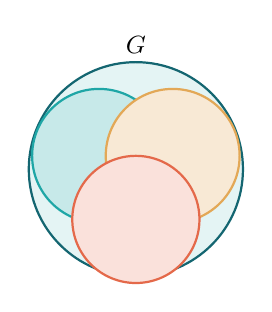
\begin{tikzpicture}[scale=0.85]
  \draw[reefMid,thick,fill=reefBright!12] (0,0) circle (1.6);
  \draw[reefBright,thick,fill=reefBright!25] (-0.55,0.2) circle (1.0);
  \draw[reefGold,thick,fill=reefGold!25] (0.55,0.2) circle (1.0);
  \draw[reefCoral,thick,fill=reefCoral!20] (0,-0.75) circle (0.95);
  \node at (0,1.85) {\small$G$};
\end{tikzpicture}
\end{column}
\end{columns}
\vspace{6pt}
\textbf{This work} extends \emph{Velasquez-Berroteran (2022)} \cite{vb} — which built the theory and classified groups up to order 60 — along three parallel strands:
\begin{center}
\small
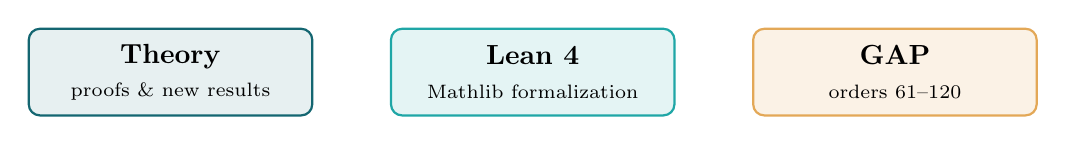
\begin{tikzpicture}
\node[draw=reefMid,thick,rounded corners,fill=reefMid!10,minimum width=3.6cm,minimum height=1.1cm,align=center] (t) at (0,0) {\textbf{Theory}\\ \scriptsize proofs \& new results};
\node[draw=reefBright,thick,rounded corners,fill=reefBright!12,minimum width=3.6cm,minimum height=1.1cm,align=center] (l) at (4.6,0) {\textbf{Lean 4}\\ \scriptsize Mathlib formalization};
\node[draw=reefGold,thick,rounded corners,fill=reefGold!15,minimum width=3.6cm,minimum height=1.1cm,align=center] (g) at (9.2,0) {\textbf{GAP}\\ \scriptsize orders 61--120};
\end{tikzpicture}
\end{center}
\end{frame}

\begin{frame}{Preliminaries: Coverings}{Definitions 2.1--2.3, 2.6}
\begin{block}{Covering \& covering number}
A \textbf{covering} of $G$ is $\Pi = \{H_i\}$, proper subgroups with $G = \bigcup_i H_i$.
$\sigma(G)$ = min. size of a covering ($\sigma(G)=\infty$ if $G$ cyclic).
\end{block}
\begin{exampleblock}{Equal covering \& equal covering number}
$\Pi$ is an \textbf{equal covering} if all $|H_i|$ coincide. $\eps(G)$ = min. size of an equal covering ($\eps(G) = \infty$ if none exists).
\end{exampleblock}
\begin{alertblock}{Partition}
$\Pi$ is a \textbf{partition} if members intersect pairwise trivially; $\rho(G)$ its minimum size. Since every equal partition is an equal covering,
\[
\eps(G) \le \rho(G).
\]
\end{alertblock}
\vspace{4pt}
Also used throughout: $\exp(G) = \operatorname{lcm}\{|g| : g\in G\}$, and $G = H\rtimes K$ (semidirect product, $H\trianglelefteq G$, $HK=G$, $H\cap K=1$).
\end{frame}

% ================= SECTION: THEORY =================
\section{Theoretical Results}

\begin{frame}{Foundational Theorems}{Proved in full to complete the framework of \cite{vb}}
\begin{columns}[T]
\begin{column}{0.5\textwidth}
\begin{block}{Theorem (Covering exists $\iff$ non-cyclic)}
$G$ has a covering iff $G$ is non-cyclic.
\end{block}
\vspace{2pt}
\textit{Idea:} a generator would force $H=G$; conversely $\{\langle a\rangle : a\in G\}$ covers.
\end{column}
\begin{column}{0.5\textwidth}
\begin{block}{Theorem ($\sigma(G)\ne 2$)}
No group is a union of two proper subgroups.
\end{block}
\vspace{2pt}
\textit{Idea:} if $h\in H\setminus K,\, k\in K\setminus H$, then $hk$ lies in neither $H$ nor $K$ — contradiction.
\end{column}
\end{columns}
\vspace{8pt}
\begin{exampleblock}{Proposition}
$2 < \sigma(G) \le n-1$, via the covering by all cyclic subgroups of non-identity elements.
\end{exampleblock}
\end{frame}

\begin{frame}{Scorza's Theorem (1926)}{$\sigma(G)=3 \iff G/N \cong C_2\times C_2$}
\begin{block}{Statement}
$\sigma(G) = 3$ \; iff \; there exists $N \trianglelefteq G$ with $G/N \cong C_2\times C_2$.
\end{block}
\textbf{Proof sketch ($\Rightarrow$).} Given a minimal 3-cover $H_1,H_2,H_3$:
\begin{enumerate}
\item Show all pairwise intersections coincide: $N := H_1\cap H_2 = H_1\cap H_3 = H_2\cap H_3$ (else a product $hh_3$ escapes the covering).
\item Set $X_i := H_i\setminus N$. Show $X_i\cdot X_j = X_k$ and $X_i\cdot X_i = N$.
\item Conclude $\{N,X_1,X_2,X_3\}$ is a Klein four-group, so $N\trianglelefteq G$, $G/N\cong C_2\times C_2$.
\end{enumerate}
\vspace{4pt}
\begin{alertblock}{Why it matters}
This is the template argument reused throughout \S3: control the intersection structure, then read off the quotient.
\end{alertblock}
\end{frame}

\begin{frame}{Haber--Rosenfeld Theorem}{Covering by the least prime divisor}
Let $p$ be the smallest prime divisor of $|G|$.
\begin{block}{(i) Lower bound}
$G$ cannot be covered by $p$ or fewer proper subgroups.
\end{block}
\textit{Proof idea:} $|G| < \sum|H_i| \le n\cdot|H_{\max}| \le n\cdot\frac{|G|}{p}$ forces $n > p$.
\begin{block}{(ii) Structure at $p+1$ subgroups}
If $\Pi$ covers $G$ with exactly $p+1$ subgroups, some $H_i$ has index $p$; if that $H_i \trianglelefteq G$, then \emph{every} member has index $p$, and $p^2 \mid |G|$.
\end{block}
\textit{Proof idea:} counting via $HH_i = G$ and inclusion–exclusion on indices rules out all-larger-index configurations.
\end{frame}

\begin{frame}{Covering-Sum Inequality \& Multiplicativity}{Lemmas 3.7--3.9}
\begin{columns}[T]
\begin{column}{0.5\textwidth}
\begin{block}{Covering-sum inequality}
\[
\sum_{i=1}^n \frac{1}{[G:H_i]} \ge 1
\]
\end{block}
\begin{exampleblock}{Quotient monotonicity}
$N\trianglelefteq G \;\Rightarrow\; \sigma(G) \le \sigma(G/N)$ \\
\scriptsize (pull back a minimal cover of $G/N$ along $\pi$)
\end{exampleblock}
\end{column}
\begin{column}{0.5\textwidth}
\begin{alertblock}{Products}
$\sigma(H\times K) \le \min\{\sigma(H),\sigma(K)\}$, with \textbf{equality} when $\gcd(|H|,|K|)=1$.
\end{alertblock}
\vspace{2pt}
\scriptsize\textit{Key fact used:} coprimality forces every subgroup $L\le H\times K$ to split as $L = \pi_H(L)\times\pi_K(L)$ (via Bézout).
\end{column}
\end{columns}
\end{frame}

\begin{frame}{Equal Covering Theorems}{Statements from \cite{vb}, reproved \& formalized}
\begin{columns}[T]
\begin{column}{0.5\textwidth}
\begin{itemize}
\item[\textbf{Thm 13}] Equal covering $\Rightarrow \exp(G)\mid |H_i|$ for all $i$.
\item[\textbf{Cor 1}] $\exp(G)\nmid |K|$ for every maximal $K$ $\Rightarrow$ no equal covering.
\item[\textbf{Thm 14}] $D_{2n}$ has an equal covering $\iff n$ is even.
\item[\textbf{Thm 15}] Every non-cyclic finite $p$-group has one.
\end{itemize}
\end{column}
\begin{column}{0.5\textwidth}
\begin{itemize}
\item[\textbf{Thm 16}] If $G$ or $H$ has one, so does $G\times H$.
\item[\textbf{Thm 17}] Every non-cyclic nilpotent group has one.
\item[\textbf{Thm 18}] Squarefree $|G|$ $\Rightarrow$ no equal covering.
\item[\textbf{Thm 19}] $N\trianglelefteq G$, $G/N$ has one $\Rightarrow$ so does $G$; likewise if $G=H\rtimes K$ and $K$ does.
\end{itemize}
\end{column}
\end{columns}
\vspace{6pt}
\begin{block}{Role in this project}
Theorem 13 is the master constraint driving both the GAP search space (\S5) and the alternating-group argument (\S6).
\end{block}
\end{frame}

% ================= SECTION: LEAN =================
\section{Lean 4 Formalization}

\begin{frame}{Lean 4 Formalization: Overview}{Self-contained algebraic core}
\begin{columns}[T]
\begin{column}{0.55\textwidth}
\textbf{Formalized (both directions where relevant):}
\begin{itemize}
\item Thm 1 — covering $\iff$ non-cyclic
\item Thm 2 — $\sigma(G)\ne 2$
\item Thm 13 — $\exp(G)\mid|H_i|$
\item Cor 1 — exponent obstruction
\item Thm 16 — equal covering of $G\Rightarrow G\times H$
\item Thm 19 — pullback along a surjection
\end{itemize}
\small Thms 15, 17 stated as \texttt{axiom}s with correct type signatures, pending full proof.
\end{column}
\begin{column}{0.45\textwidth}
\textbf{Core definitions built:}
\begin{itemize}
\item \texttt{Group}, \texttt{IsSubgroup}, \texttt{Subgroup}
\item \texttt{Covering}, \texttt{EqualCovering}
\item \texttt{order\_subgroup}, \texttt{exp}, \texttt{order\_elem}
\item \texttt{MaxSubgroup}, \texttt{divides\_max}
\item \texttt{DirectProduct}, \texttt{ProdSubgroup}
\item \texttt{Homomorphism}, \texttt{Surjective}, \texttt{PreimageSubgroup}
\end{itemize}
\end{column}
\end{columns}
\end{frame}

\begin{frame}[fragile]{Representative Lean Code}{Theorem 2: $\sigma(G) \ne 2$}
\begin{block}{Structure of the formal proof}
\begin{itemize}
\item Assume a covering $H \cup K = G$ (as a totality of the disjunction).
\item Extract witnesses $k \notin H$, $h\notin K$ from properness.
\item Case on $h\cdot k \in H$ vs.\ $h\cdot k \in K$; cancel to force $k\in H$ or $h\in K$ — contradiction either way.
\end{itemize}
\end{block}
\begin{center}
\begin{minipage}{0.92\textwidth}
\footnotesize
\ttfamily
theorem theorem2 (G) (H K : Subgroup G) (pH : IsProper H) (pK : IsProper K) :\\
\ \ Not (forall x, H.subset x \textbackslash{}/ K.subset x) := by\\
\ \ intro covers\\
\ \ rcases pH with ⟨k, hk\_notH⟩;\ rcases pK with ⟨h, hh\_notK⟩\\
\ \ have h\_mul\_k := covers (G.mul h k)\\
\ \ cases h\_mul\_k with\\
\ \ \ | inl hin =>\ have := cancel\_lemma H h k hh\_notK hin;\ contradiction\\
\ \ \ | inr kin =>\ have := cancel\_lemma2 K h k hk\_notH kin;\ contradiction
\end{minipage}
\end{center}
\end{frame}

\begin{frame}{Formalization Challenges}{Where paper mathematics resists Lean}
\begin{itemize}
\item \textbf{Axiomatizing vs.\ importing.} A self-contained \texttt{Group}/\texttt{Subgroup} core (not Mathlib's) keeps the file readable, but re-axiomatizes Lagrange's theorem and the exponent–order relation instead of reusing Mathlib proofs.
\item \textbf{Order as type vs.\ number.} Initial \texttt{Size : Subgroup G $\to$ Type u} sidestepped finiteness; switched to numeric \texttt{order\_subgroup : Subgroup G $\to$ Nat} for Thm 13+, which required threading finiteness hypotheses through every later lemma.
\item \textbf{Case-heavy classical proofs.} Scorza's theorem needs \texttt{Classical.byContradiction} and explicit witness extraction — easy on paper, delicate without decidability.
\item \textbf{No quotient groups yet.} Theorem 19 required building \texttt{PreimageSubgroup} from scratch; full Thm 19(ii) via $G=H\rtimes K$ is future work.
\end{itemize}
\end{frame}

% ================= SECTION: GAP =================
\section{GAP Computational Investigation}

\begin{frame}{The Algorithm}{Extending the search from order 60 to order 120}
\begin{columns}[T]
\begin{column}{0.55\textwidth}
\begin{block}{\texttt{HasEqualCovering(G)}}
\begin{enumerate}
\item If $G$ cyclic $\to$ \textbf{false} (Thm 1).
\item \texttt{CandidateOrders}: divisors $d\mid|G|$, $d<|G|$, $\exp(G)\mid d$ (Thm 13 prunes the search).
\item Bucket all subgroups by order.
\item For each candidate $d$: test whether that bucket's subgroups cover $G$ (bitset over elements).
\end{enumerate}
\end{block}
\end{column}
\begin{column}{0.45\textwidth}
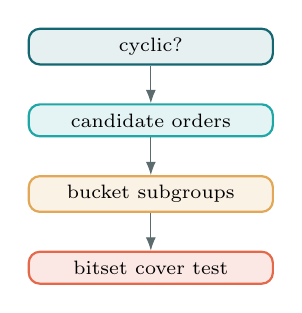
\begin{tikzpicture}[scale=0.72,every node/.style={font=\scriptsize}]
\node[draw=reefMid,thick,rounded corners,fill=reefMid!10,minimum width=3.1cm] (a) at (0,3) {cyclic?};
\node[draw=reefBright,thick,rounded corners,fill=reefBright!12,minimum width=3.1cm] (b) at (0,1.7) {candidate orders};
\node[draw=reefGold,thick,rounded corners,fill=reefGold!15,minimum width=3.1cm] (c) at (0,0.4) {bucket subgroups};
\node[draw=reefCoral,thick,rounded corners,fill=reefCoral!15,minimum width=3.1cm] (d) at (0,-0.9) {bitset cover test};
\draw[-{Latex},reefGrey] (a)--(b);
\draw[-{Latex},reefGrey] (b)--(c);
\draw[-{Latex},reefGrey] (c)--(d);
\end{tikzpicture}
\end{column}
\end{columns}
\vspace{4pt}
\textit{Exponent pruning (Theorem 13) is the essential optimization} — it collapses the divisor search from all of $\operatorname{Div}(|G|)$ to only multiples of $\exp(G)$.
\end{frame}

\begin{frame}{Results: Orders 61--120}{Complete classification, consistent with theory}
\begin{columns}[T]
\begin{column}{0.55\textwidth}
\begin{itemize}
\item Every group of order $61$--$120$ tested; result recorded as \textbf{cyclic}, \textbf{yes}, or \textbf{no}.
\item Order $64$ ($2^6$): \textbf{all} 267 non-cyclic groups admit an equal covering — consistent with Theorem 15 ($p$-groups).
\item Order $120$: mixed — includes $S_5$, $\mathrm{SL}(2,5)$, $C_2\times A_5$, all \textbf{no} equal covering (simple/near-simple composition factors).
\item Squarefree orders (e.g.\ $66,70,102,110$): uniformly \textbf{no}, matching Theorem 18.
\end{itemize}
\end{column}
\begin{column}{0.45\textwidth}
\small
\begin{tabular}{lll}
\toprule
Order & Groups & Notable \\
\midrule
64 & 267 & all \textbf{Yes} \\
72 & 50 & mixed \\
96 & 231 & mixed \\
108 & 45 & mixed \\
120 & 47 & incl.\ $S_5$, $\mathrm{SL}(2,5)$ \\
\bottomrule
\end{tabular}
\end{column}
\end{columns}
\begin{alertblock}{Consistency check}
No exception to Theorems 13--19 was found in the extended range; every ``no'' case is explained by an exponent or squarefree obstruction.
\end{alertblock}
\end{frame}

\begin{frame}{Challenges \& Patterns}
\begin{block}{Challenges}
\begin{itemize}
\item Runtime grows sharply with $|G|$ — subgroup enumeration and bitset coverage checks needed optimization to reach order 120.
\item Extending toward simple groups generally is infeasible here: \cite{vb} already verified the conjecture computationally up to order $10{,}000$.
\end{itemize}
\end{block}
\begin{exampleblock}{Patterns observed}
\begin{itemize}
\item Results are fully consistent with Theorems 13--19 across the extended range.
\item Every simple group encountered has \textbf{no} equal covering — further evidence for Conjecture 1.1.
\end{itemize}
\end{exampleblock}
\end{frame}

% ================= SECTION: CONJECTURE =================
\section{The Simple Group Conjecture}

\begin{frame}{Conjecture 1.1 and Known Evidence}
\begin{block}{Conjecture (Velasquez-Berroteran, 2022)}
If $G$ is a finite simple group, then $G$ has no equal covering.
\end{block}
\begin{itemize}
\item Verified computationally in \cite{vb} for all finite simple groups of order $< 100{,}000$.
\item \textbf{Proposition 6.2.} If $G$ is finite, non-cyclic, simple, and $\exp(G) = |G|/2$, then $G$ has no equal covering.
\end{itemize}
\begin{alertblock}{Why quotients don't help here}
Simple groups have no nontrivial normal subgroups, so Theorem 19 (transfer from $G/N$) is vacuous. Any equal covering must come entirely from internal subgroup structure, constrained by Theorem 13.
\end{alertblock}
\end{frame}

\begin{frame}{New Contribution: Alternating Groups $A_p$}{Toward the conjecture for prime degree}
\begin{block}{Conjecture 6.4 (this work)}
For every prime $p \ge 5$, the alternating group $A_p$ has no equal covering.
\end{block}
\textbf{Proof strategy.} Suppose $A_p$ has an equal covering $\{H_i\}$.
\begin{enumerate}
\item By Theorem 13, $\exp(A_p) \mid |H_i|$ for every $i$.
\item Since $p \mid \exp(A_p)$, every $H_i$ contains a Sylow $p$-subgroup of $A_p$ (order $p$).
\item \textbf{Route A:} show this forces some Sylow $p$-subgroup to be normal in $A_p$ $\Rightarrow$ contradicts simplicity.
\item \textbf{Route B:} show no maximal subgroup of $A_p$ can contain a Sylow $p$-subgroup at all $\Rightarrow$ no valid $H_i$ exists.
\end{enumerate}
\begin{alertblock}{Status}
Both routes reduce to the Sylow structure and maximal-subgroup lattice of $A_p$ — a concrete, tractable target left as the immediate next step.
\end{alertblock}
\end{frame}

% ================= SECTION: CONCLUSION =================
\section{Conclusion}

\begin{frame}{Conclusion \& Future Directions}
\begin{columns}[T]
\begin{column}{0.52\textwidth}
\textbf{Contributions:}
\begin{itemize}
\item Full proofs of Haber--Rosenfeld and all core equal-covering theorems of \cite{vb}.
\item A new partial result toward Conjecture 1.1: a Sylow-theoretic strategy for $A_p$, $p$ prime.
\item Lean 4 formalization of 6 key theorems, with 2 stated as axioms pending proof.
\item GAP classification extended from order 60 to order 120 — fully consistent with theory.
\end{itemize}
\end{column}
\begin{column}{0.44\textwidth}
\textbf{Future work:}
\begin{itemize}
\item Complete the Lean proofs of Theorems 15 and 17.
\item Push Conjecture 6.4 to a full proof for $A_p$, $p\ge 5$ prime.
\item Extend GAP classification beyond order 120.
\end{itemize}
\vspace{10pt}
\begin{center}
{\color{reefMid}\Large\headingfont\bfseries Thank you}
\end{center}
\end{column}
\end{columns}
\end{frame}

% ================= REFERENCES =================
\begin{frame}{References}
\footnotesize
\begin{thebibliography}{9}
\bibitem{gap} \textit{GAP -- Groups, Algorithms, Programming}. \url{https://www.gap-system.org/}
\bibitem{lean} \textit{Lean 4}. \url{https://lean-lang.org/}
\bibitem{cohn} J.\,H.\,E.\ Cohn. \textit{On n-sum groups.}
\bibitem{hr} S.\ Haber, A.\ Rosenfeld. \textit{Groups as unions of proper subgroups.} Amer.\ Math.\ Monthly \textbf{66}:491--494.
\bibitem{scorza} G.\ Scorza. \textit{Bollettino Unione Matematica Italiana.}
\bibitem{vb} A.\ Velasquez-Berroteran. \textit{Equal Coverings of Finite Groups.} 2022.
\end{thebibliography}
\end{frame}

\end{document}